\documentclass{beamer}
\usecolortheme{beaver}

\usepackage[utf8]{inputenc}

\usepackage{graphicx}
\usebackgroundtemplate%
{%
    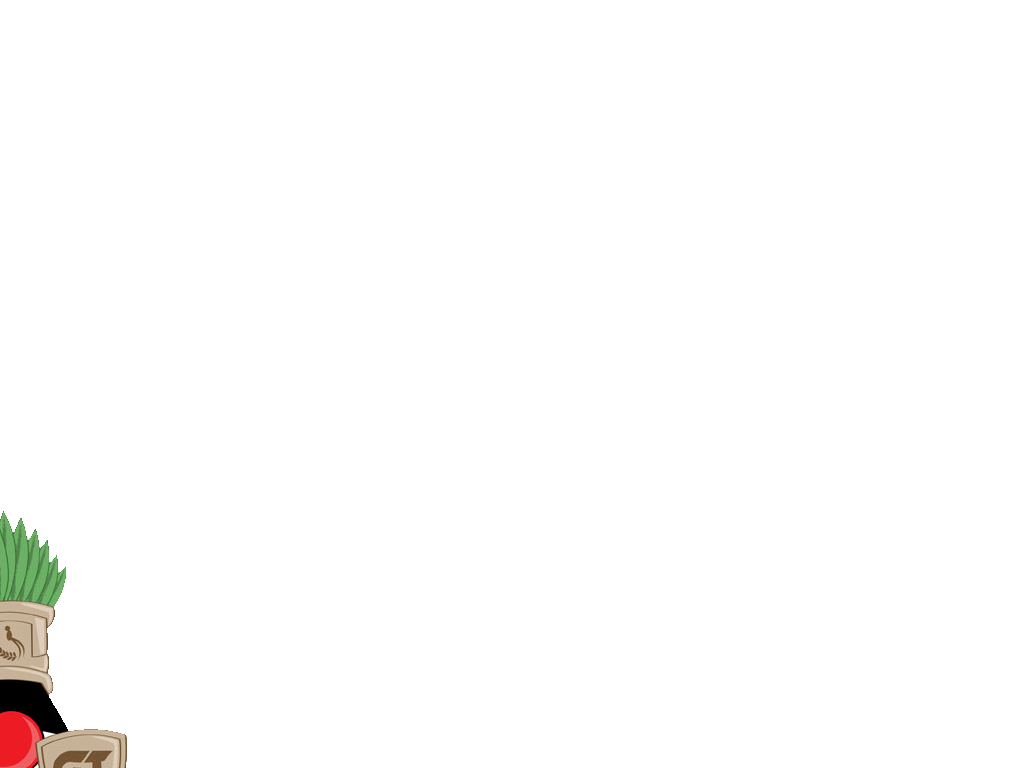
\includegraphics[width=\paperwidth]{Images/fondoguatejug}%
}

\title{Creando aplicaciones Web con AngularJS y JavaEE 7}
\author{Víctor Orozco}
\institute{Nabenik}
\date{\today}

\begin{document}

\frame{\titlepage}

\section{Intro}

\begin{frame}{Víctor Orozco}
     \begin{columns}[T] % contents are top vertically aligned
	     \begin{column}[T]{5cm} % each column can also be its own environment
				\begin{itemize}
				\item Developer (JVM/Open Source Advocate)
				\item Consultor independiente (Nabenik)
				\item \href{https://twitter.com/tuxtor}{GuateJUG}
				\item \href{https://twitter.com/tuxtor}{@tuxtor}
				\item \href{http://vorozco.com}{The J*} 
				\end{itemize}
	     \end{column}
	     \begin{column}[T]{5cm} % alternative top-align that's better for graphics
			\begin{figure}
			\centering
			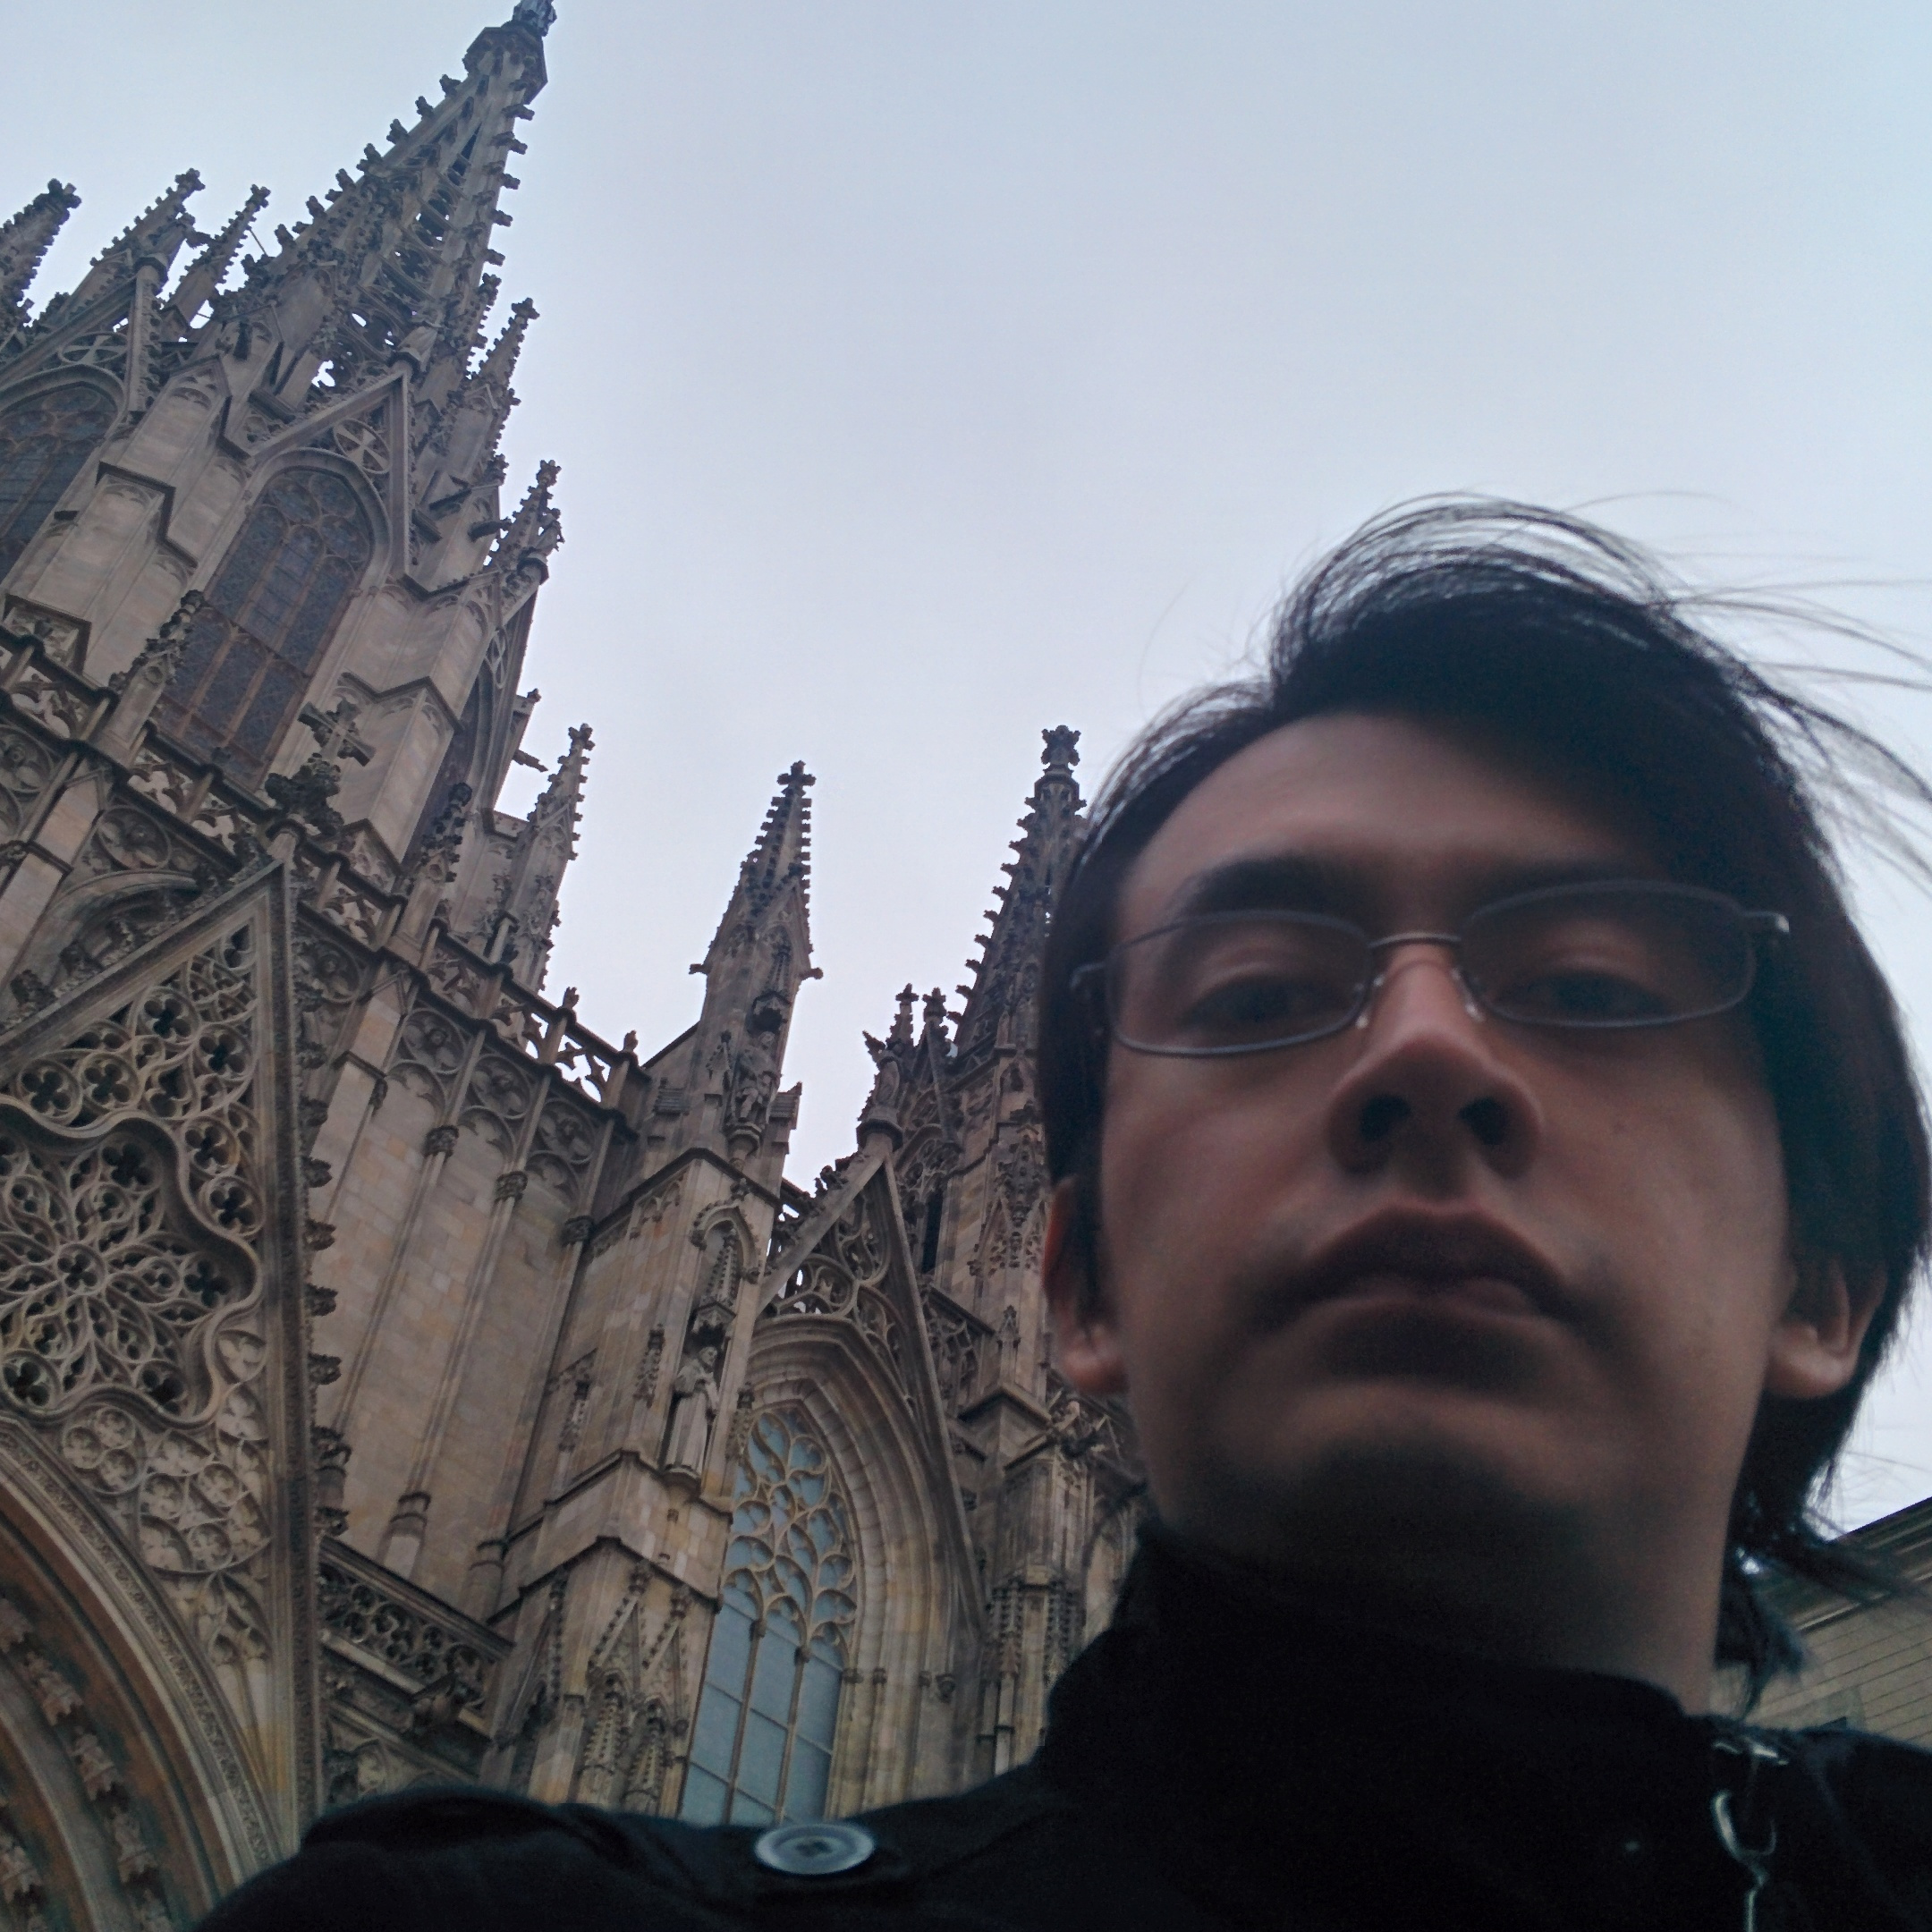
\includegraphics[width=0.7\linewidth]{Images/barcelona.jpg}
			\end{figure}

	     \end{column}
     \end{columns}
\end{frame}

\begin{frame}{Cliente/servidor}
\begin{figure}
\centering
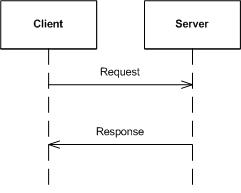
\includegraphics[width=0.5\linewidth]{Images/requestresponse}
\label{fig:requestresponse}
\end{figure}
\pause HTTP/1.1 = protocolo asíncrono y sin estado para transmitir texto
\end{frame}

\begin{frame}{Cliente/servidor}
	\begin{figure}
	\centering
	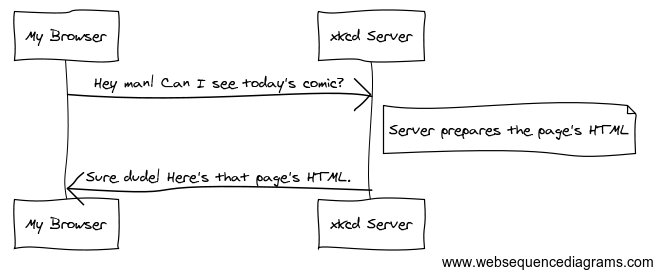
\includegraphics[width=0.8\linewidth]{Images/http-xkcd}
	\label{fig:http-xkcd}
	\end{figure}
	\pause
	\begin{itemize}
	\item Request -$>$ (HTML) -$>$ Response
	\item Servidor: PHP, JSP, ASP
	\item Servidor Java: JSP/Servlets, JSF, Struts, Spring MVC
	\end{itemize}
\end{frame}

\begin{frame}{Cliente/servidor}
	\begin{figure}
\centering
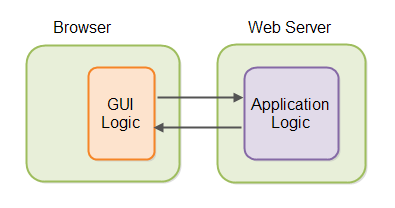
\includegraphics[width=0.7\linewidth]{Images/ria}
\label{fig:ria}
\end{figure}
	\pause
	\begin{itemize}
	\item Rich clients/RIA = obsolesencia?
	\item Request -$>$ (App) -$>$ Response
	\item Cliente: ActiveX, Applets, Flash, Silverlight, JavaFX
	\end{itemize}
\end{frame}

\begin{frame}{Clientes JavaScript}
	\begin{itemize}
	\item AJAX
	\item jQuery, YUI, Dojo
	\end{itemize}
	...
	\begin{itemize}
	\item GWT, Icefaces/Primefaces, Vaadin
	\item HTML5, CSS3, WebSockets, WebRTC, HTML Components
	\end{itemize}
\end{frame}

\begin{frame}{Clientes JavaScript}
	1995-2012: JavaScript SUCKS! - Developer Foo con conocimientos de otro lenguaje que no sea JS.
		\begin{itemize}
			\item Orientado a hacks
			\item Imperativo (manipulación DOM)
			\item CoffeeScript, Dart, Kotlin, RapydScript, TypeScript, AtScript
			\item MVVM (su buen vecino MS)
		\end{itemize}
	2012-2015: JavaScript SUCKS . . . less
\end{frame}

\begin{frame}{Clientes JavaScript/HTML5}
		\begin{itemize}
			\item Rich clients = HTML+JS+CSS3
			\item MVVM +- MVC del lado del cliente
			\item JSON/XML
			\item Rest - Request-response
			\item Websockets - Full duplex
		\end{itemize}
\end{frame}

\section{JS}
\begin{frame}{Arquitectura 2015}
	\begin{figure}
\centering
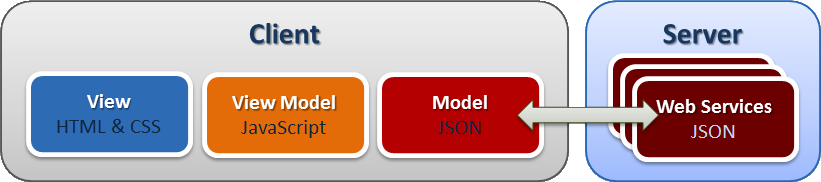
\includegraphics[width=0.9\linewidth]{Images/arq2015b}
\end{figure}
\end{frame}

\begin{frame}{Arquitectura 2015}
	\begin{figure}
\centering

\includegraphics[width=0.8\linewidth]{Images/embernode.png}
\end{figure}
\end{frame}

\begin{frame}{Arquitectura 2015}
	\begin{figure}
\centering

\includegraphics[width=0.8\linewidth]{Images/knockoutnet.png}
\end{figure}
\end{frame}

\begin{frame}{Arquitectura 2015}
	\begin{figure}
\centering

\includegraphics[width=0.8\linewidth]{Images/anguaree.png}
\end{figure}
\end{frame}

\begin{frame}{AngularJS}
	\begin{itemize}
		\item AngularJS fue creado por desarrolladores Java, estamos en familia :) \footnotemark[1]
		\item Inyección de dependencias
		\item Data binding
		\item Directives, partial layouts
		\item SPI
		\item JS puro (AngularJS 1)
		\item Clientes hibridos (moviles) - Cordova + AngularJS
	\end{itemize}
	\footnotetext[1]{http://java.dzone.com/articles/java-origins-angular-js}
\end{frame}

\begin{frame}{JavaEE 7}
	\begin{itemize}
		\item API Rest - JAX-RS 2.0
		\item WebSocket - WebSocket 1.0, Servlet 3.1
		\item JSON - JSON API 1.0
		\item SOA, Microservices
	\end{itemize}
	\begin{figure}
\centering
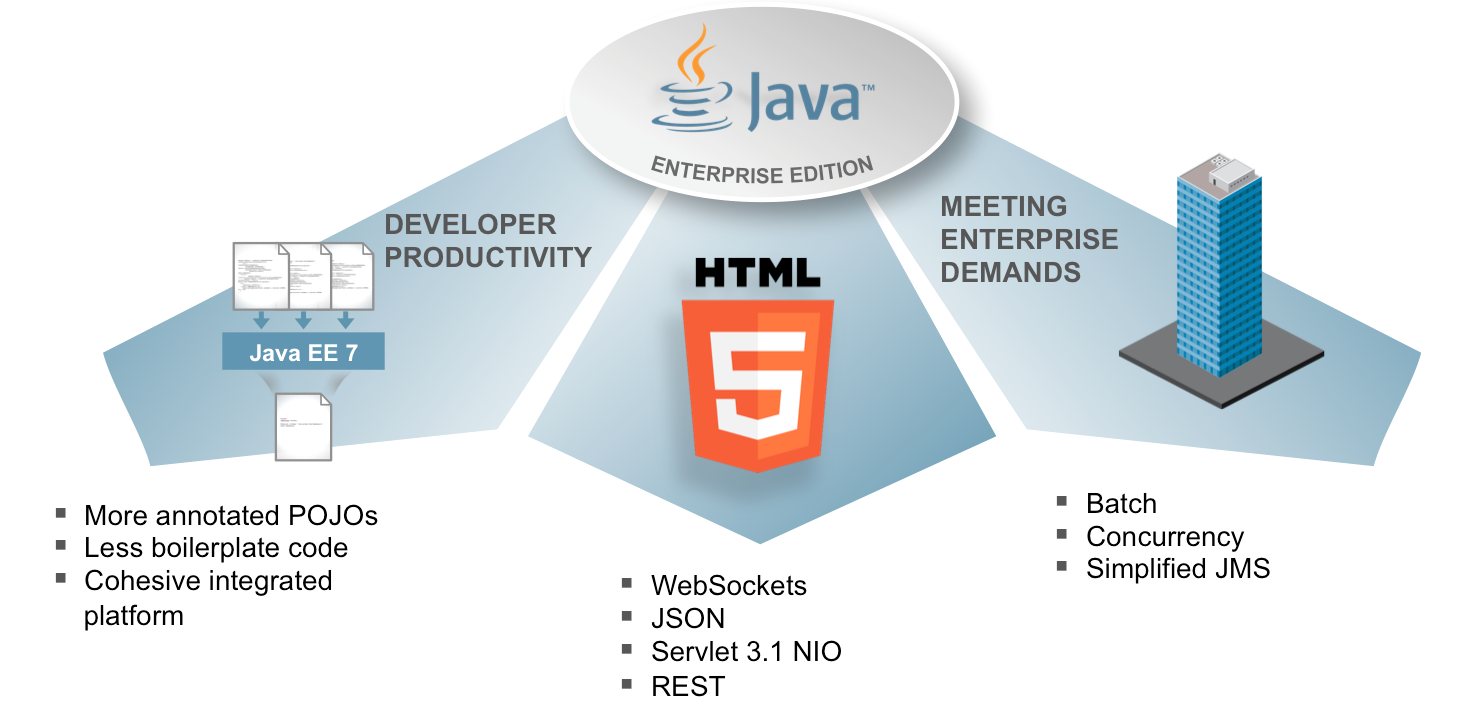
\includegraphics[width=0.7\linewidth]{Images/javaee7-theme}
\end{figure}

\end{frame}

\begin{frame}{JavaEE 7}
	\begin{figure}
\centering
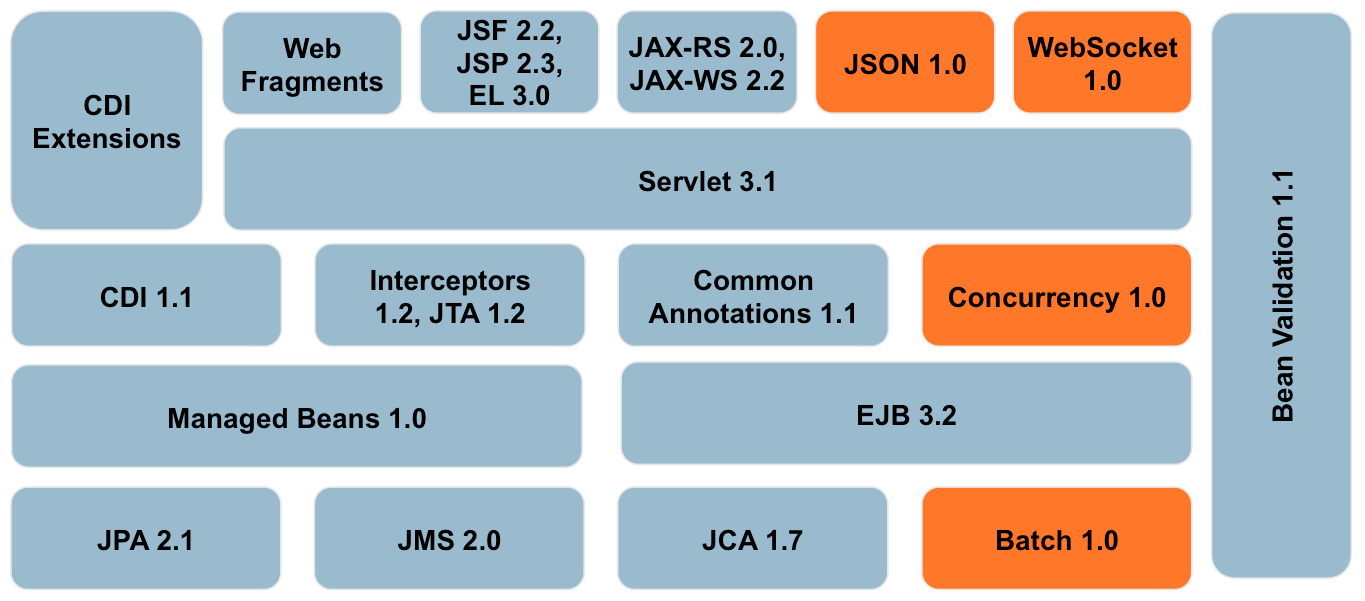
\includegraphics[width=0.9\linewidth]{Images/javaee7-pancake.png}
\end{figure}

\end{frame}

\begin{frame}{JavaEE 7}
	\begin{figure}
\centering
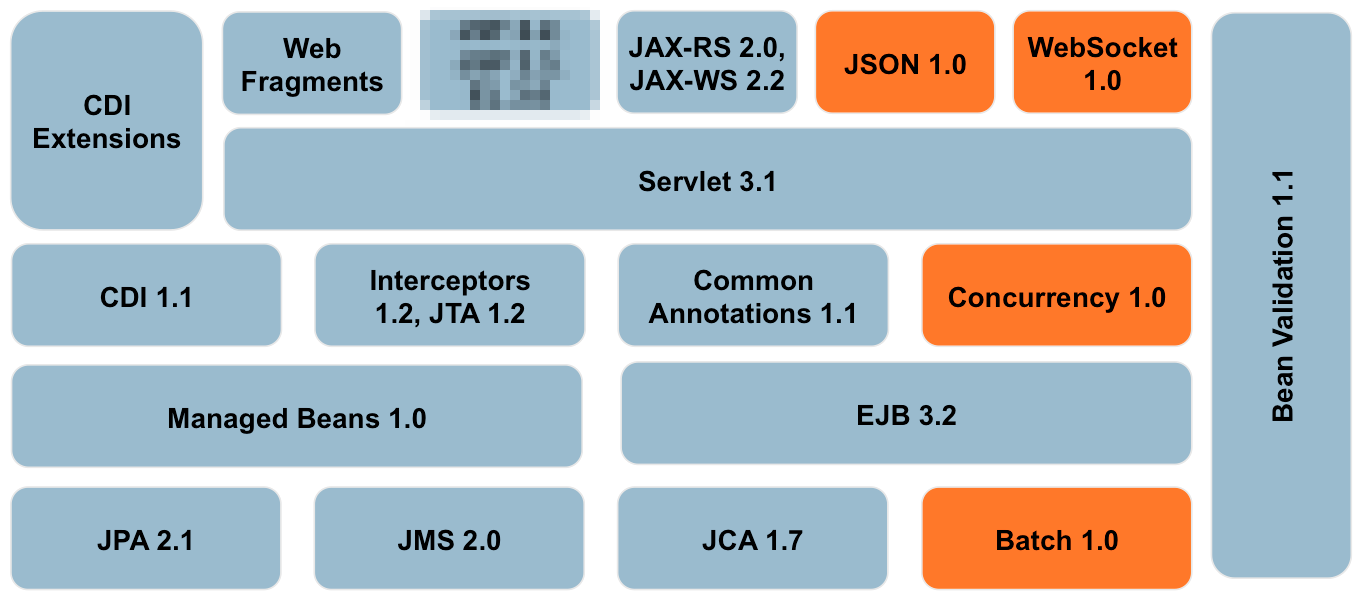
\includegraphics[width=0.9\linewidth]{Images/javaee7-modern-pancake.png}
\end{figure}
\end{frame}

\begin{frame}{Ventajas}
	\begin{itemize}
		\item Existen n cantidad de bibliotecas JavaScript
		\item Independencia de backend
		\item Escalabilidad (stateless)
		\item Thin server apps
		\item Mejor tiempo de respuesta en comparación a JSF/SpringMVC
	\end{itemize}
\end{frame}

\begin{frame}{Desventajas}
	\begin{itemize}
		\item Existen n cantidad de bibliotecas JavaScript
		\item Complejidad y restricciones de REST
		\item AngularJS no sera compatible hacia atrás
	\end{itemize}
\end{frame}

\begin{frame}{Demo}
	\begin{itemize}
		\item Call for papers
		\item H2 + WildFly
		\item Bean Validation, JPA, JAX-RS, JSON
		\item AngularJS vanilla
		\item Forge
		\item http://github.com/tuxtor/cfp-angularjs-demo
	\end{itemize}
\end{frame}

\begin{frame}{QA}
	\begin{itemize}
		\item AngularJS - https://angularjs.org/
		\item JavaEE - http://docs.oracle.com/javaee/7/index.html
		\item Libros recomendados:
		\begin{itemize}
			\item Java EE 7 Essentials - Arun Gupta
			\item Developing RESTful Services with JAX-RS 2.0 - Masoud Kalali, Bhakti Mehta
			\item Eloquent JavaScript - Marijn Haverbeke
		\end{itemize}
	\end{itemize}
\end{frame}



\section{Fin}

\begin{frame}{Gracias}
\begin{itemize}
\item tuxtor@shekalug.org
\item http://tuxtor.shekalug.org
\item http://github.com/tuxtor/slides
\end{itemize}
\begin{center}

\includegraphics[width=0.1\linewidth]{Images/cclogo}
\\
This work is licensed under a Creative Commons Attribution-ShareAlike 3.0 Guatemala License.
\end{center}
\end{frame}
\end{document}
